\documentclass[../../main.tex]{subfiles}
\graphicspath{{../../image/}{../../figure/}}
\begin{document}

\section{运动学}\label{section:ch02-运动学}

ambient 空间是 $\mathbb{R}^{m}$，维数为一、二或三。我们将使用两份 $\mathbb{R}^{m}$，一份作为\emph{参考空间}，另一份作为\emph{物理空间}。一个物体由一个\emph{参考构型}来标识，即参考空间的一个开子集 $\mathscr{B}$。$\mathscr{B}$ 的点称为\emph{质点}。典型质点记为 $x$，时间记为 $t$。

\begin{definition}[放置与运动]\label{definition:ch02-放置与运动}
物体的一个\emph{放置}是指其参考构型 $\mathscr{B}$ 到物理空间中某一开子集的一个双 Lipschitz 同胚。物体在时间区间 $(t_{1},t_{2})$ 上的一个\emph{运动}是指一个 Lipschitz 映射 $\chi:\mathscr{B}\times(t_{1},t_{2})\to\mathbb{R}^{m}$，它对每个固定的 $t\in(t_{1},t_{2})$ 的限制是一个放置。
\end{definition}

于是，对固定的 $x\in\mathscr{B}$ 和 $t\in(t_{1},t_{2})$，$\chi(x,t)$ 指定了时刻 $t$ 质点 $x$ 在物理空间中的位置；对固定的 $t\in(t_{1},t_{2})$，映射 $\chi(\cdot,t):\mathscr{B}\to\mathbb{R}^{m}$ 给出物体在时刻 $t$ 的放置；最后，对固定的 $x\in\mathscr{B}$，曲线 $\chi(x,\cdot):(t_{1},t_{2})\to\mathbb{R}^{m}$ 描述了质点 $x$ 在物理空间中的轨迹。见\cref{figure:ch02-运动示意图}。

\begin{figure}[ht]
\centering
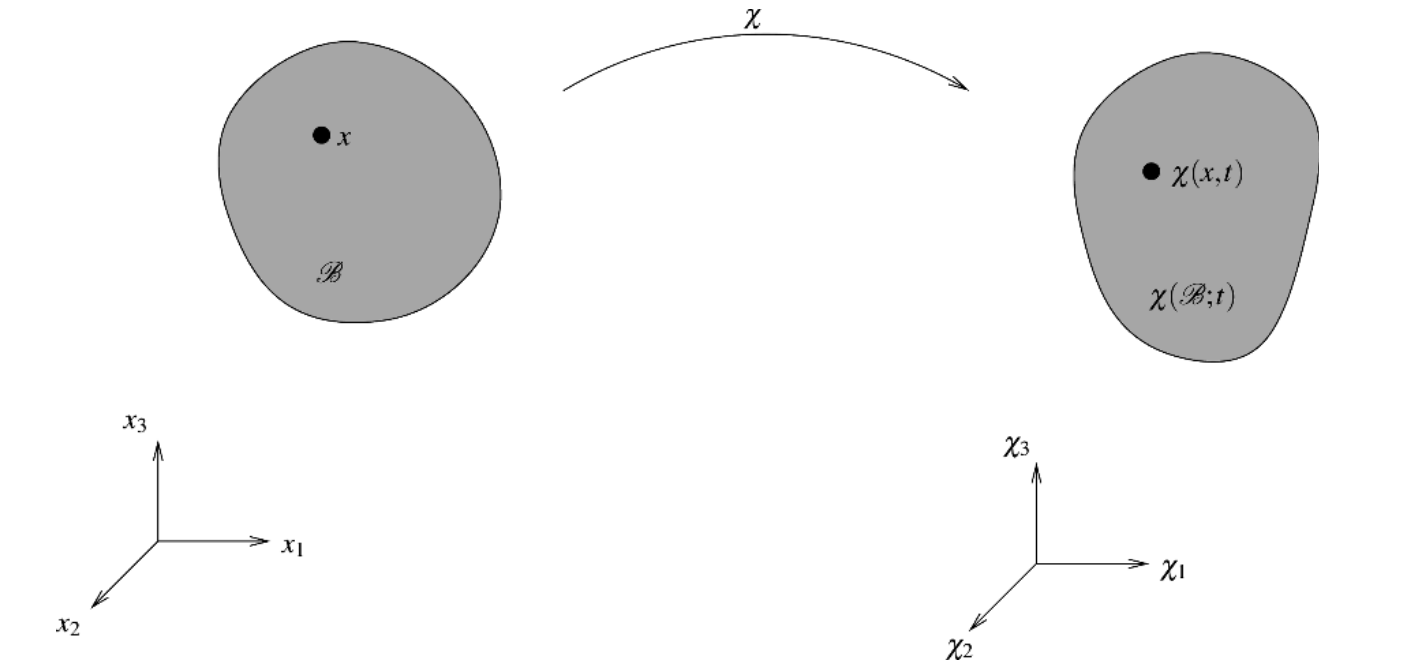
\includegraphics[width=0.85\textwidth]{ch02-fig01-01.png}
\caption{物体 $\mathscr{B}$ 的参考构型与当前放置 $\chi(\mathscr{B};t)$，以及参考坐标系 $(x_{1},x_{2},x_{3})$ 与空间坐标系 $(\chi_{1},\chi_{2},\chi_{3})$。}
\label{figure:ch02-运动示意图}
\end{figure}

参考构型一般给出物体的一个抽象表示。但在实际中，人们常常将参考空间与物理空间等同起来，并以物体的一个实际放置作为参考构型，即将物质质点与它们在该特定放置中所占的物理空间点等同起来。

连续介质物理的目标是监测物体所伴随的各种场的演化，例如密度、应力、温度等等。在\emph{参考描述}或\emph{Lagrange 描述}中，人们沿质点轨迹跟踪场的演化；而在\emph{空间描述}或\emph{Euler 描述}中，人们在空间中固定位置监测场的演化。运动使我们能够从一种描述过渡到另一种描述。例如，考察某个说明性的场 $w$，我们记 $w=f(x,t)$ 为其参考描述，记 $w=\phi(\chi,t)$ 为其空间描述。运动将 $f$ 与 $\phi$ 联系起来：$\phi(\chi(x,t),t)=f(x,t)$，其中 $x\in\mathscr{B}$，$t\in(t_{1},t_{2})$。

两种描述各有其相对优点，因此在此都将使用。于是，为了保持适当的记账，对每个场需要三个符号：一个标识该场，一个用于其参考描述，一个用于其空间描述（在上例中即 $w$、$f$ 和 $\phi$）。然而，为了控制符号的膨胀并使方程的物理意义透明，标准的记号约定是用场的同一标识符号承担全部三种用途。为避免记号在导数上的歧义，将采用以下规则：关于 $t$ 的偏导数在参考描述中用头顶点号表示，在空间描述中用 $t$ 下标表示。梯度、微分和散度\footnote{为与矩阵记号一致，梯度实现为 $m$ 维列向量，微分实现为 $m$ 维行向量，即梯度的转置。如第 I 章一样，散度算子作用于行向量。}关于物质变量 $x$ 分别记为 $\mathrm{Grad}$、$\mathrm{grad}$、$d$ 和 $\mathrm{div}$，关于空间变量 $\chi$ 分别记为 $\nabla$、$d$ 和 $\mathrm{div}$。于是，再以典型场 $w$ 为例，其参考描述为 $w=f(x,t)$，空间描述为 $w=\phi(\chi,t)$，则 $\dot{w}$ 表示 $\partial f/\partial t$，$w_{t}$ 表示 $\partial\phi/\partial t$，$\mathrm{Grad}\,w$ 表示 $\mathrm{grad}_{x}f$，$\mathrm{grad}\,w$ 表示 $\mathrm{grad}_{\chi}\phi$。这种记号初看可能令人困惑，但本学科的学生很快就能学会高效而正确地使用它。

运动 $\chi$ 诱导出两个重要的运动学场，即速度
\begin{align}
v=\dot{\chi},
\label{align:ch02-2-1-1}
\end{align}
属于 $L^{\infty}(\mathscr{B}\times(t_{1},t_{2});\mathbb{R}^{m})$；以及\emph{变形梯度}，顾名思义，它是运动的微分：
\begin{align}
F=\nabla\chi,
\label{align:ch02-2-1-2}
\end{align}
属于 $L^{\infty}(\mathscr{B}\times(t_{1},t_{2});\mathbb{M}^{m\times m})$。按照放置的定义，我们假定
\begin{align}
\det F\geqslant a>0\qquad\text{a.e.}
\label{align:ch02-2-1-3}
\end{align}

这些场使我们能够从空间导数过渡到物质导数；例如，假定 $w$ 是一个 Lipschitz 场，
\begin{align}
\dot{w}=w_{t}+(\mathrm{d}w)v,
\label{align:ch02-2-1-4}
\end{align}
\begin{align}
\mathrm{Grad}\,w=F^{\top}\mathrm{grad}\,w,\qquad\nabla w=(\mathrm{d}w)F.
\label{align:ch02-2-1-5}
\end{align}

由极分解定理，介质的局部变形（由变形梯度 $F$ 表示）可实现为一个纯拉伸与一个旋转的复合：
\begin{align}
F=RU,
\label{align:ch02-2-1-6}
\end{align}
其中对称正定矩阵
\begin{align}
U=(F^{\top}F)^{1/2}
\label{align:ch02-2-1-7}
\end{align}
称为\emph{右拉伸张量}，而正常正交矩阵 $R$ 称为\emph{旋转张量}。

转向变形的变化率，我们引入参考与空间\emph{速度梯度}（它们实际上是微分）：
\begin{align}
\dot{F}=\nabla v,\qquad L=\mathrm{d}v.
\label{align:ch02-2-1-8}
\end{align}
$L$ 分解为对称\emph{拉伸张量} $D$ 与反对称\emph{自旋张量} $W$ 之和：
\begin{align}
L=D+W,\qquad D=\tfrac{1}{2}(L+L^{\top}),\qquad W=\tfrac{1}{2}(L-L^{\top}).
\label{align:ch02-2-1-9}
\end{align}
自旋张量只是涡量向量 $\omega=\mathrm{curl}\,v$ 作为反对称矩阵的表示。

Lipschitz 连续运动这一类允许激波，但范围不够宽，不能囊括弹性中的空化、流体动力学中的涡、气体动力学中的真空等运动。即便如此，我们仍将在运动 Lipschitz 连续的假设下发展理论，将推广的考虑推迟到确有需要时再进行。

\end{document}
